\documentclass[xcolor=dvipsnames]{beamer}
\usepackage[T1]{fontenc}
\usepackage[utf8]{inputenc}
\usepackage[english,slovak]{babel}

\usepackage{amsmath}
\usepackage{amsthm}
\usetheme{Pittsburgh}
\useoutertheme{shadow}

\usepackage{graphicx}
\usepackage{caption}
\usepackage{subcaption}

\usepackage[]{algorithm2e}
\usepackage{listings}
 \setbeamercovered{transparent}
 \usepackage{cuted}
\usepackage[export]{adjustbox}
\usepackage{mathtools}

\usepackage{lipsum}
\usepackage{verbatim}
\usepackage{transparent}
\usepackage{framed}
\usepackage{xcolor}

\usepackage{multirow}
\usepackage{colortbl}

\newcommand\Wider[2][3em]{%
\makebox[\linewidth][c]{%
  \begin{minipage}{\dimexpr\textwidth+#1\relax}
  \raggedright#2
  \end{minipage}%
  }%
}




\iftrue

\usetheme{Warsaw}

\setbeamercolor{normal text}{fg=white,bg=black!90}
\setbeamercolor{structure}{fg=white}

\setbeamercolor{alerted text}{fg=red!85!black}

\setbeamercolor{item projected}{use=item,fg=black,bg=item.fg!35}

\setbeamercolor*{palette primary}{use=structure,fg=structure.fg}
\setbeamercolor*{palette secondary}{use=structure,fg=structure.fg!95!black}
\setbeamercolor*{palette tertiary}{use=structure,fg=structure.fg!90!black}
\setbeamercolor*{palette quaternary}{use=structure,fg=structure.fg!95!black,bg=black!80}

\setbeamercolor*{framesubtitle}{fg=white}

\setbeamercolor*{block title}{parent=structure,bg=black!60}
\setbeamercolor*{block body}{fg=black,bg=black!10}
\setbeamercolor*{block title alerted}{parent=alerted text,bg=black!15}
\setbeamercolor*{block title example}{parent=example text,bg=black!15}

\fi



%-------------------------------------------------------------------------------------
\title{\color{white} \bf Neural networks}
\author{\color{white} Michal CHOVANEC, PhD}


%\setbeamertemplate{footline}[frame number]{}
\setbeamertemplate{navigation symbols}{}


\date[EURP]{}
\begin{document}

{
    \usebackgroundtemplate
    {
        \vbox to \paperheight{\vfil\hbox to \paperwidth{\hfil

        {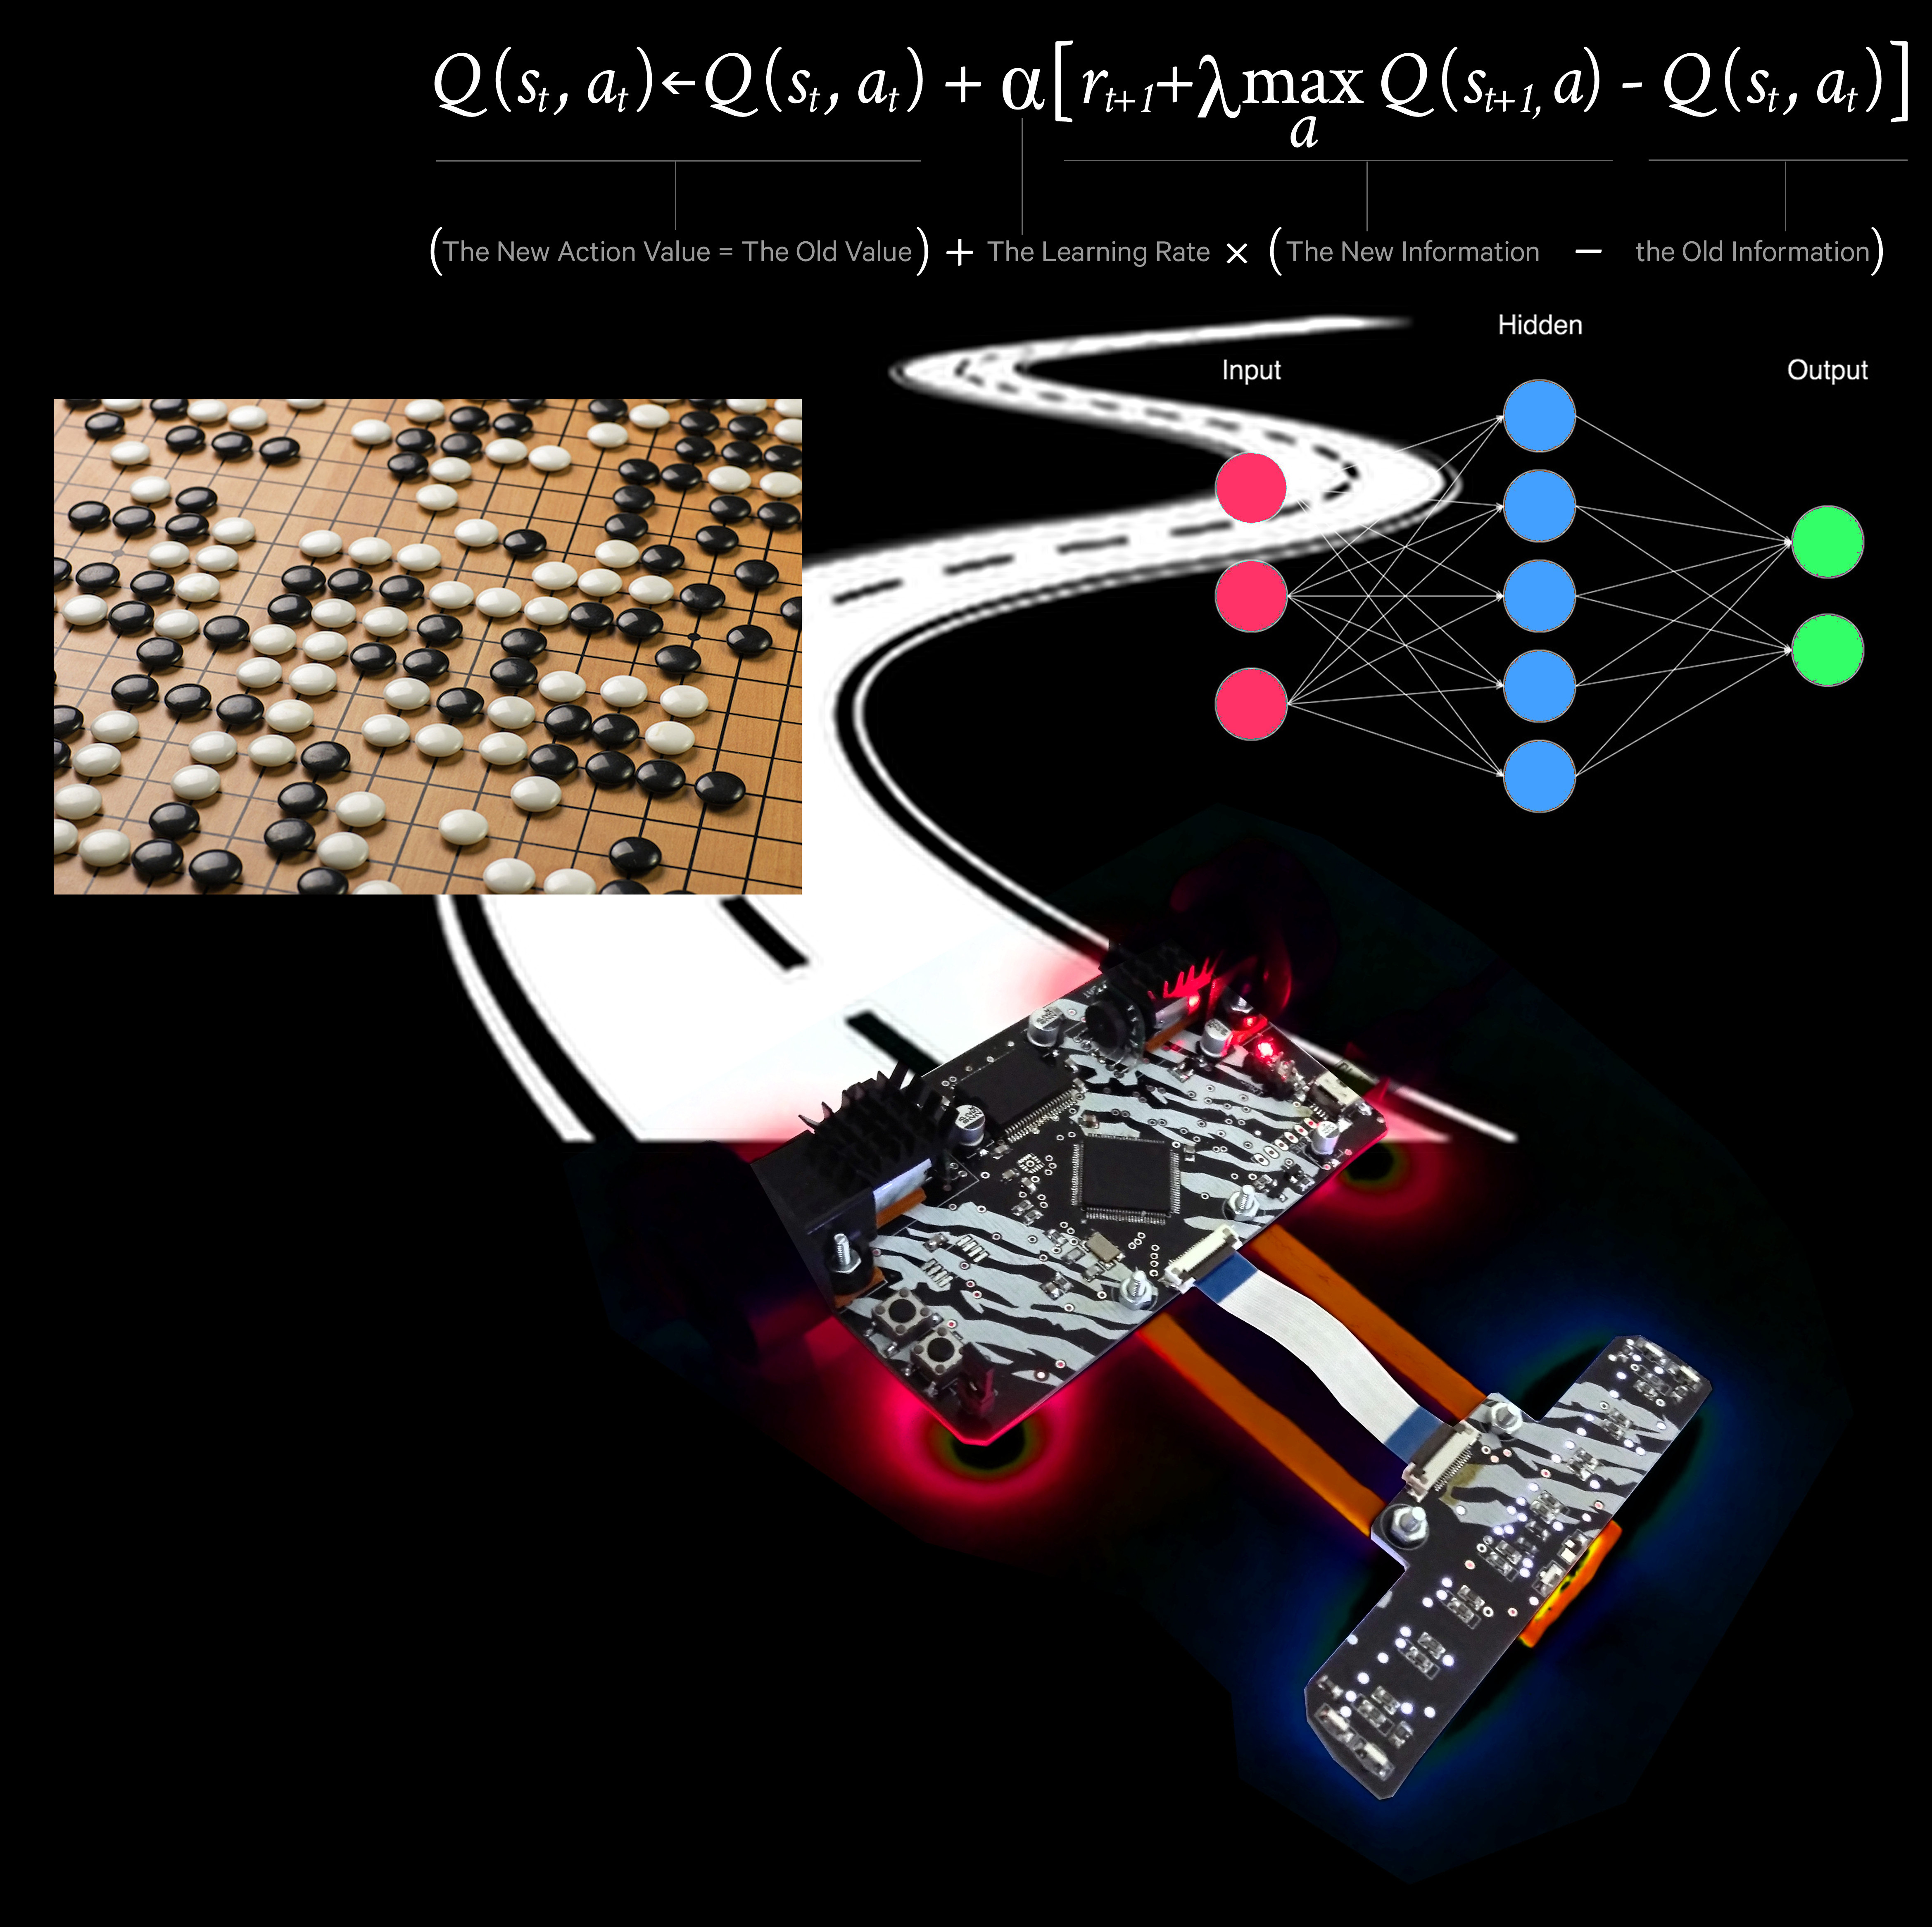
\includegraphics[width=5.05in]{../../pictures/rl_square.jpg}}

        \hfil}\vfil}
    }
    \begin{frame}

    %\titlepage


    \centering
     \colorbox{black}
     {
        \begin{minipage}{7cm}
           {\LARGE \color{white} \bf Neural networks} \\
           {\LARGE \color{white} Michal CHOVANEC, PhD} \\
       \end{minipage}
     }


    \end{frame}
}



\begin{frame}{\bf Neural network}

\begin{figure}
  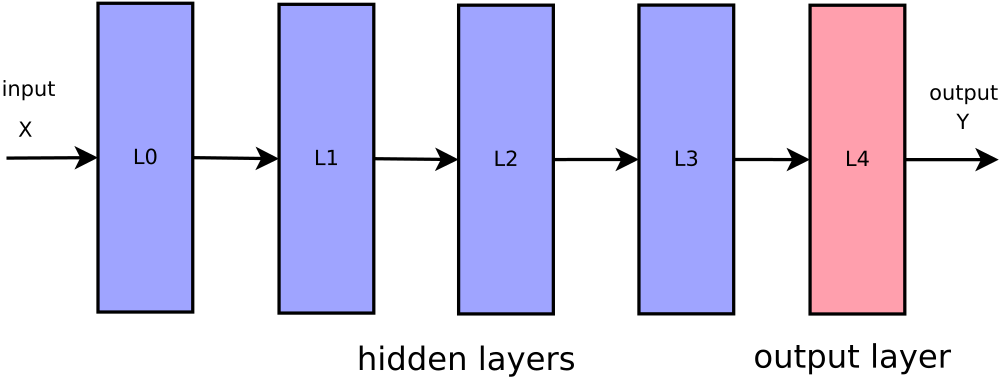
\includegraphics[scale=0.2]{../../diagrams/nn/nn.png}
\end{figure}


\begin{itemize}
  \item universal function {\bf \color{red} approximator}
  \item learning from examples
  \item training using parallel architectures {\bf \color{red} NVIDIA GPU}, TPU - from weeks to months
  \item {\bf \color{red} inspired} by human brain
  \item thousands of connected {\bf \color{red} neurons}
\end{itemize}


\end{frame}


\begin{frame}{\bf Layer}

\begin{figure}
  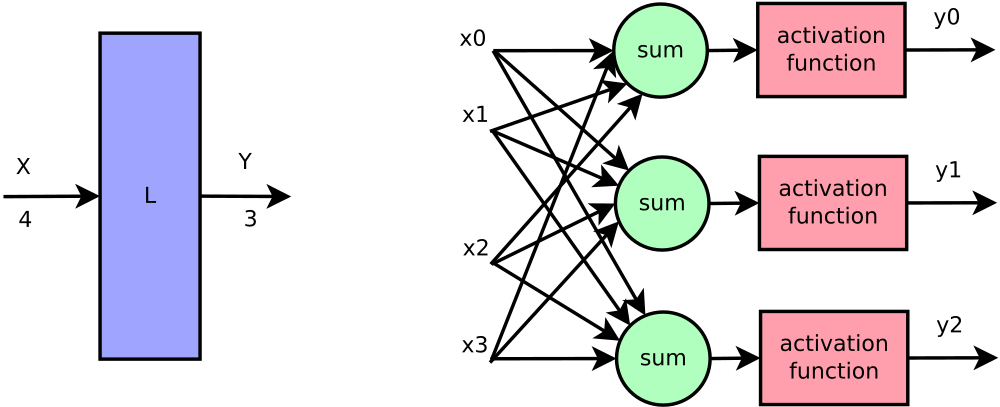
\includegraphics[scale=0.2]{../../diagrams/nn/nn_layer.png}
\end{figure}

\begin{columns}
    \begin{column}{0.5\textwidth}

    \begin{align*}
        y_j = f(\sum_{i=0}^{N-1} X_iW_{ji} + b_j) \\
    \end{align*}

    \end{column}

    \begin{column}{0.5\textwidth}  %%<--- here

    where \\
        $f(x)$ is activation function \\
        $X$ input vector \\
        $W$ weights matrix \\
        $b$ bias vector \\
        $Y$ output vector \\

    \end{column}



\end{columns}



\end{frame}




\begin{frame}{\bf Layer}

\begin{figure}
  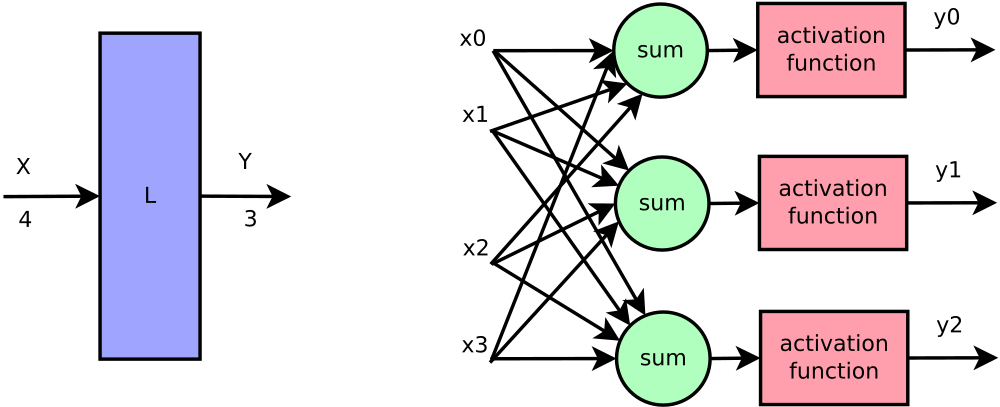
\includegraphics[scale=0.2]{../../diagrams/nn/nn_layer.png}
\end{figure}

\begin{align*}
    y_0 = f(\sum_{i=0}^{3} X_iW_{0i} + b_0) \\
    y_1 = f(\sum_{i=0}^{3} X_iW_{1i} + b_1) \\
    y_2 = f(\sum_{i=0}^{3} X_iW_{2i} + b_2) \\
\end{align*}

\end{frame}


\begin{frame}{\bf Layer - split activation function}

\begin{figure}
  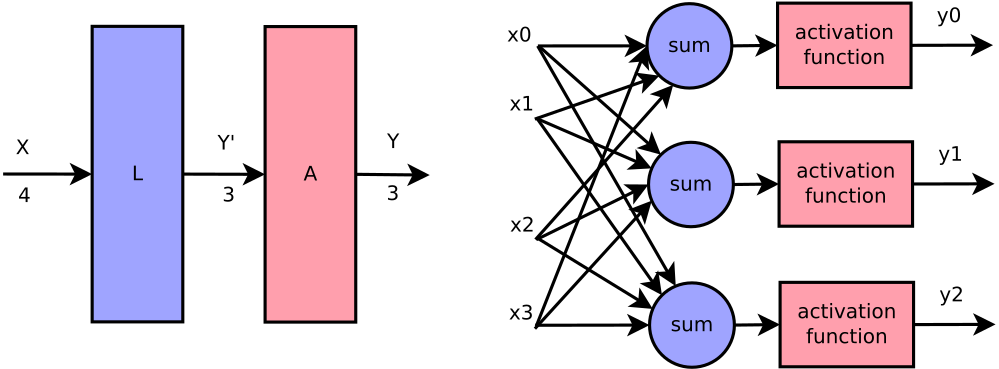
\includegraphics[scale=0.2]{../../diagrams/nn/nn_layer_split.png}
\end{figure}

\begin{align*}
    y'_0&= \sum_{i=0}^{3} X_iW_{0i} + b_0, &&y_0 = f(y'_0)\\
    y'_1&= \sum_{i=0}^{3} X_iW_{1i} + b_1, &&y_1 = f(y'_1)\\
    y'_2&= \sum_{i=0}^{3} X_iW_{2i} + b_2, &&y_2 = f(y'_2)\\
\end{align*}

$y'$ is called neuron {\bf \color{red} Activation}

\end{frame}

\begin{frame}{\bf Activation function}

\begin{table}[]
\begin{tabular}{|l|l|l|}
\hline
\textbf{name} & \textbf{function}        & \textbf{derivative} \\ \hline
{\bf \color{red} Linear}        & $y = x$                    & $y' = 1$              \\ \hline
Sigmoid       & $y = \frac{1}{1+e^{-x}}$  & $y' = \frac{e^{-x}}{(1+e^{-x})^2}$             \\ \hline
RBF           & $y = e^{-x^2}$ & $y' = xe^{-x^2}$                   \\ \hline
{\bf \color{red} Relu}          & $ y=\begin{cases} x, & \text{if $x>0$}\\ 0, & \text{otherwise} \end{cases}$ & $ y'=\begin{cases} 1, & \text{if $x>0$}\\ 0, & \text{otherwise} \end{cases}$                  \\ \hline
LeakyRelu     & $ y=\begin{cases} x, & \text{if $x>0$}\\ 0.01x, & \text{otherwise} \end{cases}$ & $ y'=\begin{cases} 1, & \text{if $x>0$}\\ 0.01, & \text{otherwise} \end{cases}$               \\ \hline
\end{tabular}
\end{table}

\begin{figure}
  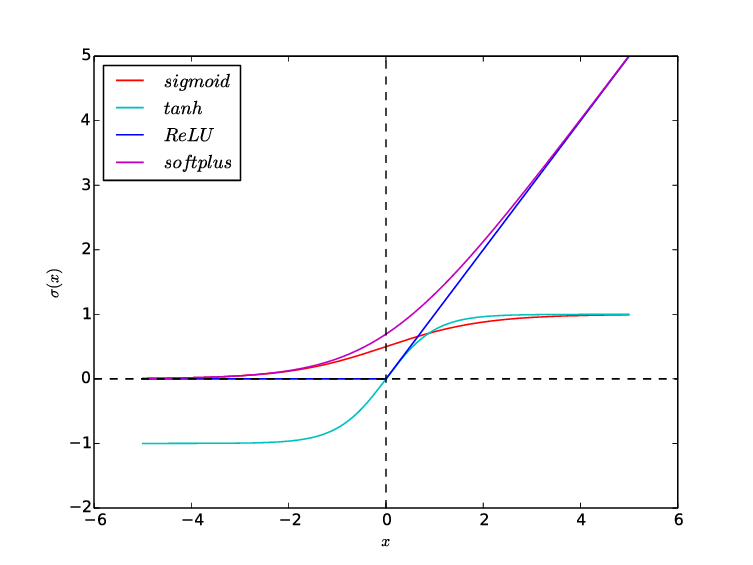
\includegraphics[scale=0.15]{../../pictures/activation.png}
\end{figure}

\end{frame}


\begin{frame}{\bf Training}

\begin{enumerate}
  \item choose random training dataset sample $(X, Y)$
  \item compute neural network output, $\hat{Y} = F(X)$
  \item obtain error\\
    error = {\bf \color{green} target value} - {\bf \color{red} computed value} \\
    $E = Y - \hat{Y}$
  \item update weights and biases using error
\end{enumerate}

\end{frame}


\begin{frame}{\bf Training}

\begin{figure}
  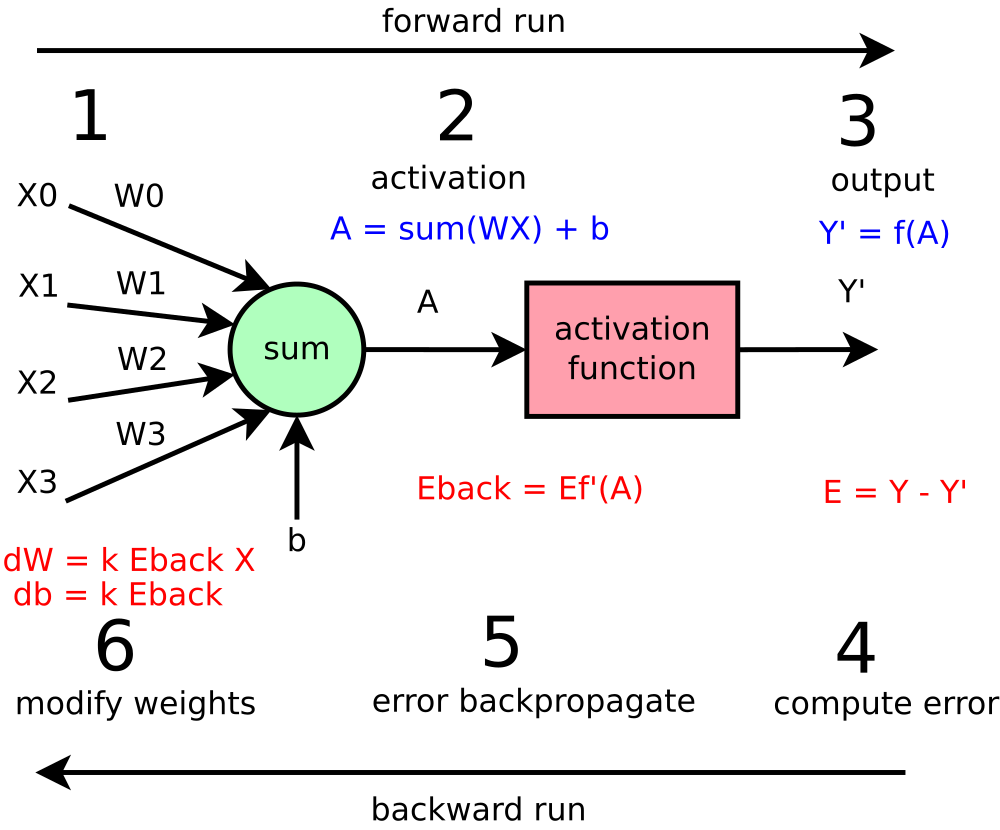
\includegraphics[scale=0.3]{../../diagrams/nn/neuron_learn.png}
\end{figure}

\end{frame}

\begin{frame}{\bf Training}
One neuron weights updating example \\
- consider $Y, \hat{Y}, b$ are scalar values, and $W, X$ are vectors
\begin{align*}
    E &= Y - \hat{Y} \\
    J &= \underset{\bf \color{red} cost\ function\ to\ minimize}{\left(Y - f(\sum_{i=0}^{N-1} X_iW_i + b) \right)^2} \\
    \frac{\partial J}{\partial W_j} &= -2 \underset{\bf \color{red} Error\ E}{\left(Y - f(\sum_{i=0}^{N-1} X_iW_i + b) \right)}f'\underset{\bf \color{red} Activation\ A}{\left(\sum_{i=0}^{N-1} X_iW_i + b\right)}X_j \\
    \frac{\partial J}{\partial W_j} &= -2Ef'(A)X_j \\
    \frac{\partial J}{\partial W_j} &\approx W_j(n) - W_j(n-1) = \Delta W_j \\
    \Delta W_j &=  \eta Ef'(A)X_j\
\end{align*}
\end{frame}

\begin{frame}{\bf Training}
special case for $y(x) = x$
    \begin{align*}
    \Delta W_j &=  \eta EX_j
    \end{align*}

special case for $y(x) = RELU(x)$
        \begin{align*}
        \Delta W_j &=
        \begin{cases}
            \eta EX_j \text{ if $\sum_{i=0}^{N-1} X_iW_{ji} + b_0 > 0$}\\
            0 \text{ otherwise} \\
        \end{cases}
        \end{align*}
\end{frame}

\begin{frame}{\bf Error backpropagation}

\begin{figure}
  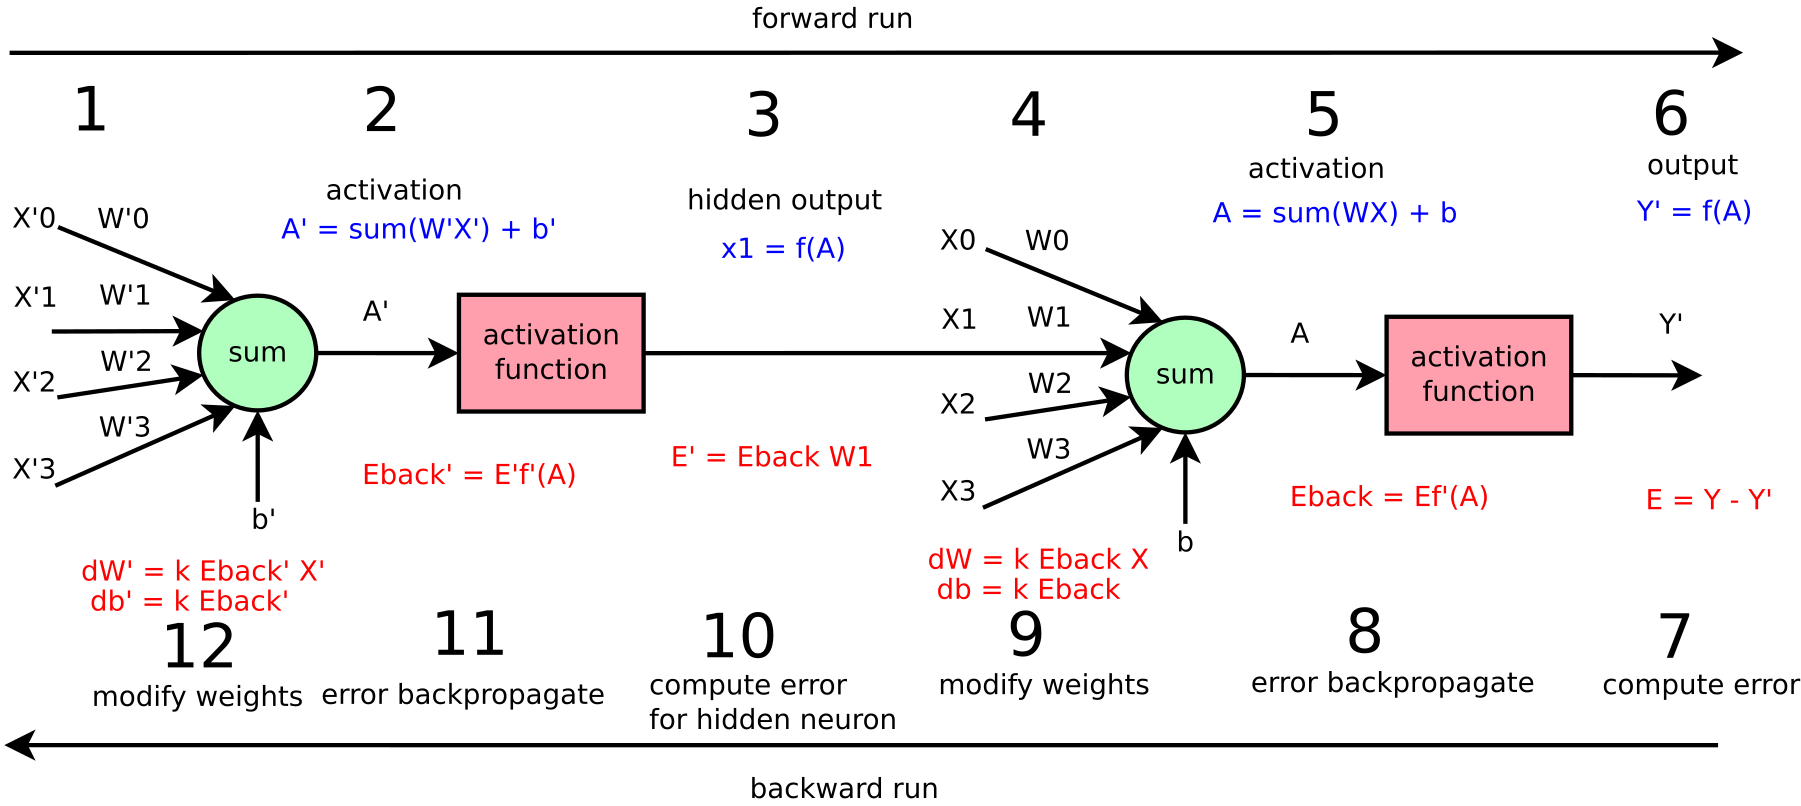
\includegraphics[scale=0.22]{../../diagrams/nn/neuron_backpropagation.png}
\end{figure}

\end{frame}


\begin{frame}{\bf Mnist handwritten numbers classification}

\begin{columns}


    \begin{column}{0.5\textwidth}

        \begin{itemize}
            \item handwritten numbers, \\
                60000 for training, \\
                10000 for testing
            \item 28x28 pixels, grayscale \\
                  9x9 pixels, mnist tiny
            \item 10 outputs
        \end{itemize}

    \end{column}

    \begin{column}{0.5\textwidth}

    \begin{figure}
      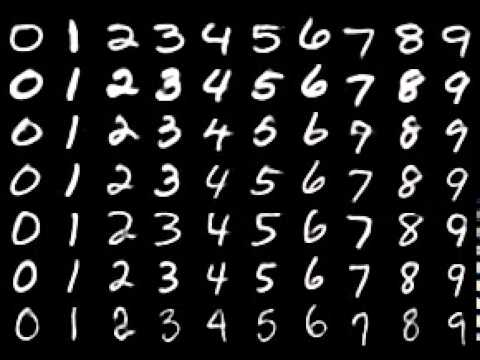
\includegraphics[scale=0.23]{../../pictures/mnist.jpg}
    \end{figure}

    \end{column}


\end{columns}


{\bf SCORING}
\begin{itemize}
\item more than 99\%  {\bf A} {\bf \color{green} best networks}
\item more than 98\%  {\bf B}  {\bf \color{blue} average networks}
\item more than 97\%  {\bf C}  {\bf \color{blue} average networks}
\item more than 96.5\%  {\bf D}   {\bf \color{red} pure networks}
\item more than 96\%  {\bf E}  {\bf \color{red} pure networks}
\item otherwise  {\bf Fx} {\bf \color{gray} linear classifier}

\end{itemize}

\end{frame}


\begin{frame}{\bf Convolutional neural networks}
\end{frame}


\begin{frame}{\bf Usefull links}

{\tiny
  \begin{thebibliography}{9}
    \bibitem {}CHRISTOPHER  J.C.H. WATKINS : Q-learning \\ \url{http://www.gatsby.ucl.ac.uk/~dayan/papers/cjch.pdf}
    \bibitem {}Richard S. Sutton : Reinforcement Learning: An Introduction \\ \url{https://www.amazon.com/Reinforcement-Learning-Introduction-Adaptive-Computation/dp/0262193981}

    \bibitem {}Google DeepMind : Playing Atari with Deep Reinforcement Learning \\ \url{https://arxiv.org/pdf/1312.5602.pdf}
    \bibitem {}Google DeepMind : Dueling Network Architectures for Deep Reinforcement Learning \\ \url{https://arxiv.org/pdf/1511.06581.pdf}
    \bibitem {}Google DeepMind :Mastering the Game of Go without Human Knowledge \\ \url{https://deepmind.com/documents/119/agz_unformatted\_nature.pdf}

    \bibitem {}Andrej Karpathy : Pong from pixels \\ \url{http://karpathy.github.io/2016/05/31/rl/}
    \bibitem {}Maxim Lapan : Deep reinforcement learning \\ \url{https://www.amazon.com/Practical-Reinforcement-Learning-Maxim-Lapan/dp/1788834240}
    \bibitem {}Mohit Sewak : Practical Convolutional Neural \\ Networks \url{https://www.amazon.com/Practical-Convolutional-Neural-Networks-Implement/dp/1788392302}
    \bibitem {}Densely Connected Convolutional Networks \\ \url{https://arxiv.org/pdf/1608.06993.pdf}
  \end{thebibliography}
}

\end{frame}


\begin{frame}{\bf Q\&A}

\begin{figure}
  
\includegraphics[scale=0.25]{../../pictures/me.jpg}
\end{figure}

\centering {
michal chovanec (michal.nand@gmail.com)
\url{www.youtube.com/channel/UCzVvP2ou8v3afNiVrPAHQGg}
}

\centering {
github
\url{https://github.com/michalnand}
}

\end{frame}


\end{document}
